\begin{frame}{Choosing the Right Comparable Area of Asia}
\vspace{-30pt}
    %\centering
\hspace{-30pt}
 \begin{minipage}{1.15\textwidth}
\begin{figure}[htb!]
    \centering
   \hspace{-40pt} 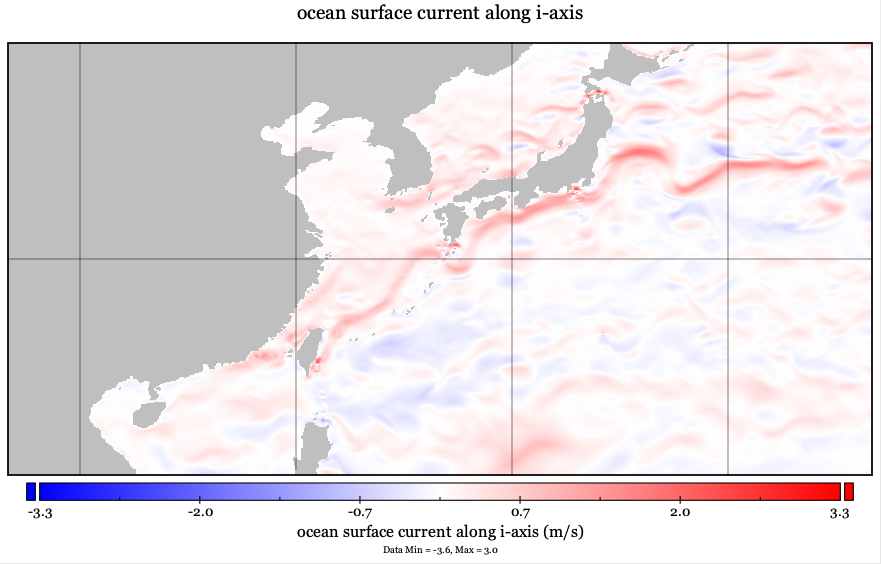
\includegraphics[width=0.42\linewidth]{images/example-images/c-uos.png}
        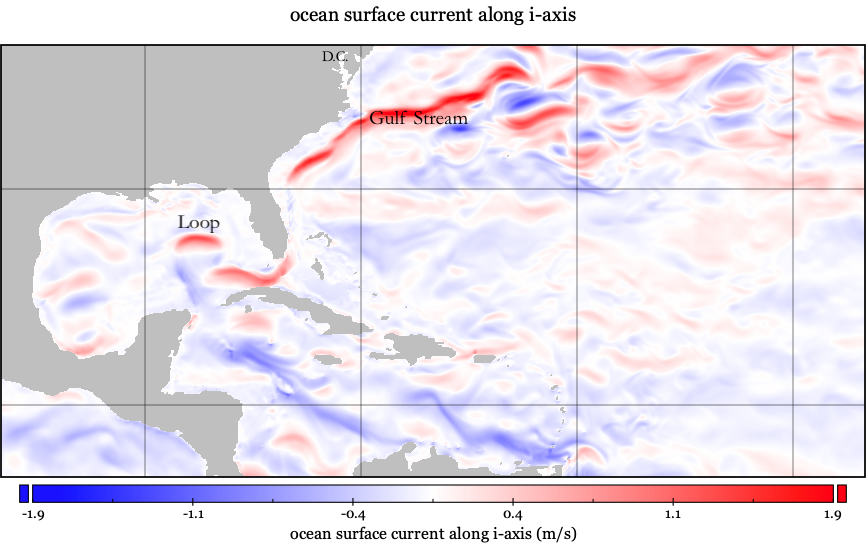
\includegraphics[width=0.42\linewidth]{images/example-images/uos.png}

   \hspace{-40pt} 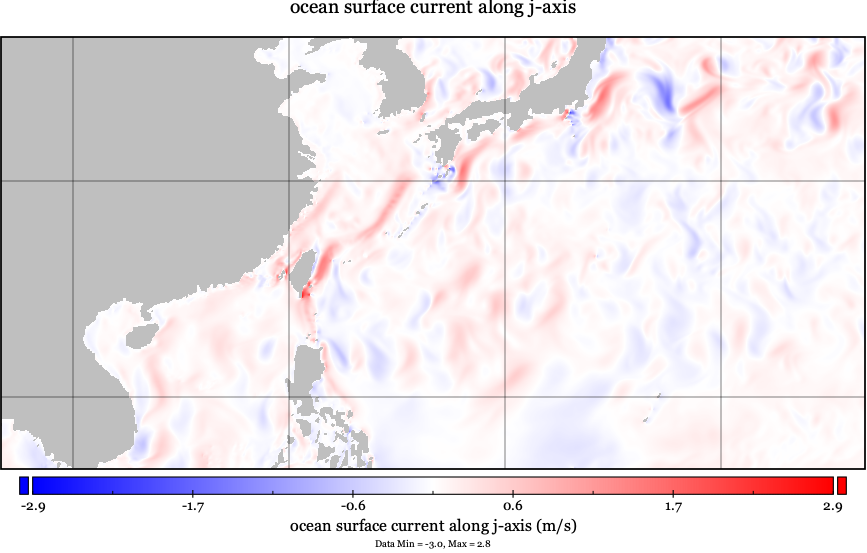
\includegraphics[width=0.42\linewidth]{images/example-images/c-vos.png}
        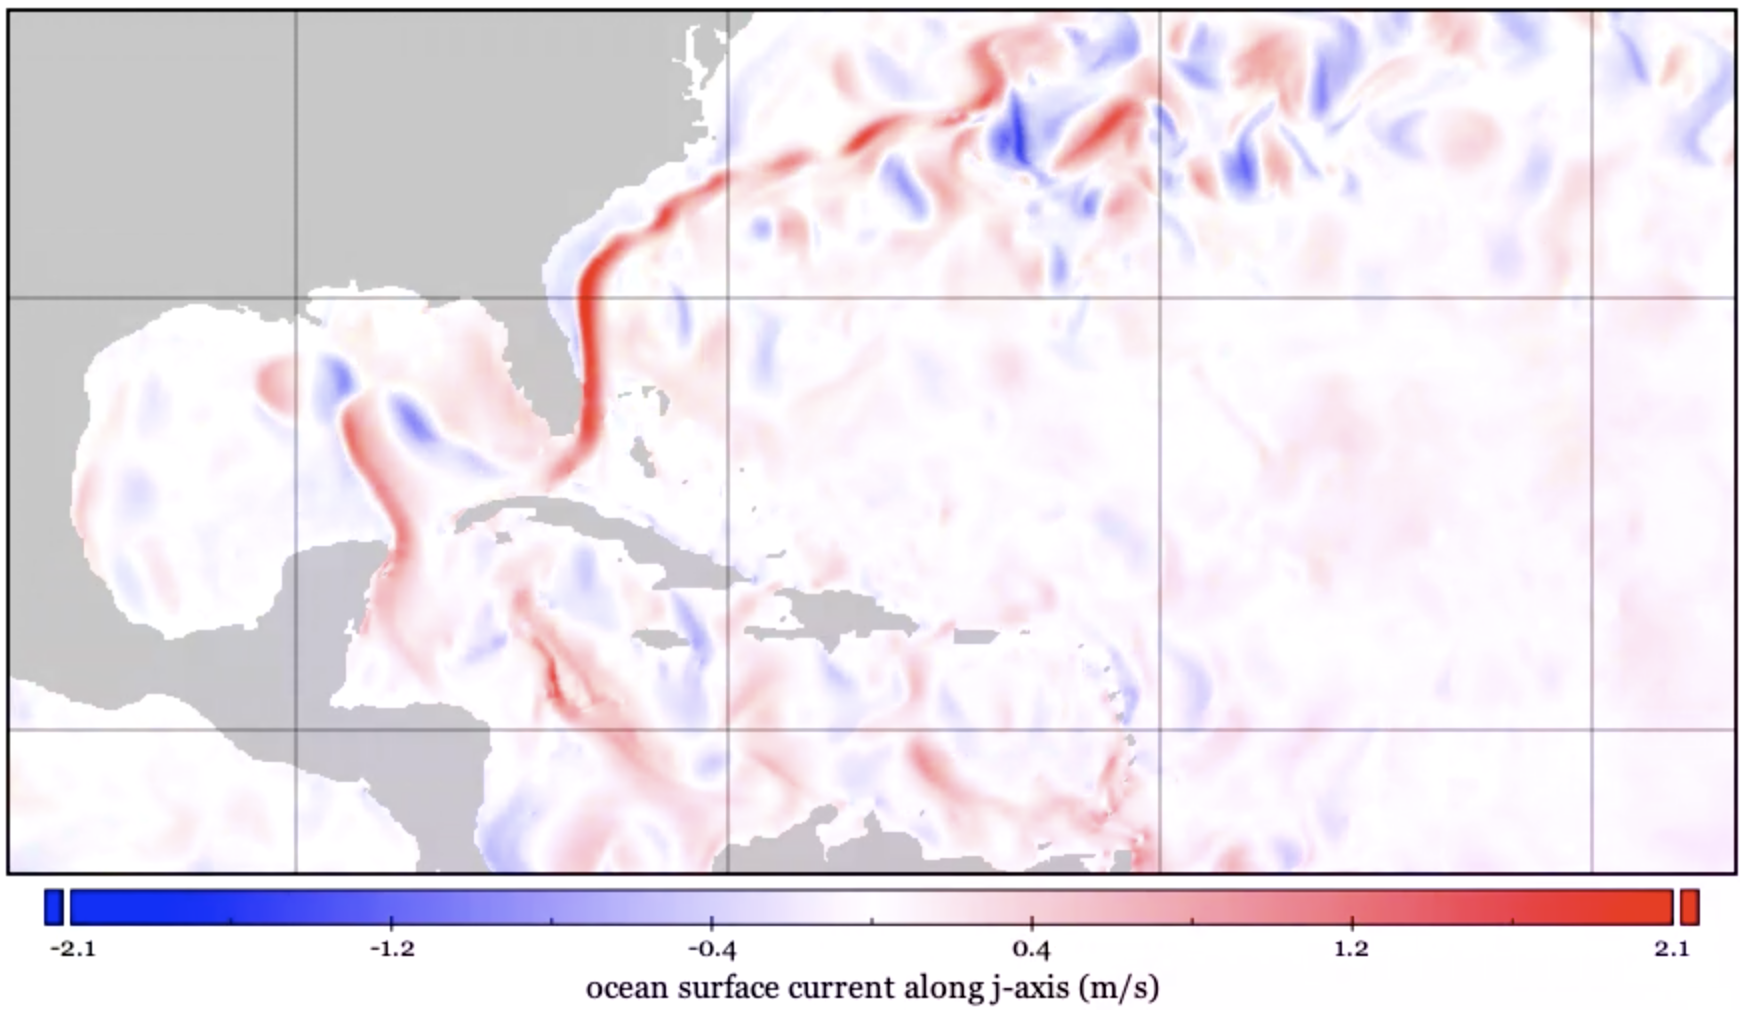
\includegraphics[width=0.42\linewidth]{images/example-images/vos.png}
    \vspace{-10pt}
    \caption{The Kuroshio and Gulf Stream share structural features.}
    \label{fig:A}
\end{figure}
\end{minipage}
\end{frame}


\begin{frame}{Helpful Coast Markers}
\vspace{-20pt}
    %\centering
 \begin{minipage}{1.0\textwidth}
\begin{figure}[htb!]
    \centering
    \includegraphics[width=0.55\linewidth]{../surge/plots/vin-china-choice.pdf}
    \vspace{-15pt}
   \caption{Automatic coastal extraction with SH island removed. }
    %\label{fig:}
\end{figure}
\end{minipage}
\end{frame}


\begin{frame}{Algorithmic Successes}
\vspace{-20pt}
    %\centering
 \begin{itemize}
\item The nearest neighbour algorithm almost flawlessly extracted the coastline
     between two points (only Shanghai island needed to be removed by hand).
\item New documentation allowed me to speed the selection scripts up by over 3 O.M.
\item This means that selecting new areas to test theories against from ORCA12
      is now a fairly trivial undertaking.
\end{itemize}
\end{frame}

\begin{frame}{VC GEV Distribution fitted to Block Maxima}
\vspace{-20pt}
    %\centering
\begin{figure}
\includegraphics[width=0.8\linewidth]{../surge/plots/vc_skextreme_second_tactic.pdf}
\caption{\cite{skextremes} }
\end{figure}
\end{frame}


\begin{frame}{VC $\eta$ (SSH/zos) similar between 2004/5 }
\vspace{-20pt}
\begin{figure}[htb!]
    \centering
    \includegraphics[width=0.6\linewidth]{../surge/plots/vc_stats/zos_moments.pdf}
       \hspace{0pt} \includegraphics[width=0.285\linewidth]{../surge/plots/vc_stats/zos_moments_dist.pdf}
    \vspace{-7pt}
    \caption{A comparison between the distributions of sea surface height
     above geoid (zos) for the training set (2005) and the test set (2004).}
   % \label{fig:}
\end{figure}
\end{frame}



\begin{frame}{VC $\eta$ Covariance and Correlation matrices. }
\vspace{-20pt}
\begin{figure}[htb!]
  \centering
  \hspace{-10pt}
  \includegraphics[width=0.68\linewidth]{../surge/plots/vc_stats/zos_corr_cov.pdf}
          \includegraphics[width=0.165\linewidth]{../surge/plots/corr_cov_cbar.pdf}
  \vspace{-7pt}
  \caption{A/B: Covariance matrices for 2004/5.\\
           $\quad\quad\quad\;\;$C/D: Correlation matrices for 2004/5.}
  \label{fig:}
\end{figure}
\end{frame}


\begin{frame}{VC $\tau_u$ Covariance and Correlation matrices. }
\vspace{-20pt}
\begin{figure}[htb!]
  \centering
  \hspace{-10pt}
  \includegraphics[width=0.68\linewidth]{../surge/plots/vc_stats/tauuo_corr_cov.pdf}
          \includegraphics[width=0.165\linewidth]{../surge/plots/corr_cov_cbar.pdf}
  \vspace{-7pt}
  \caption{A/B: Covariance matrices for 2004/5.\\
           $\quad\quad\quad\;\;$C/D: Correlation matrices for 2004/5.}
  \label{fig:}
\end{figure}
\end{frame}

\begin{frame}{VC $\eta$ Individual Points. }
\vspace{-20pt}
\begin{figure}[htb!]
  \centering
  \hspace{-10pt}
  \includegraphics[width=1\linewidth]{../surge/plots/vc_stats/zos_individual.pdf}
  \vspace{-7pt}
  \caption{There is a lack of large positive anomalies. I don't understand what
   produces so many negative anomalies further North.}
  \label{fig:}
\end{figure}
\end{frame}


\begin{frame}{VC Bathymetry. }
\vspace{-20pt}
\begin{figure}[htb!]
  \centering
  \hspace{-10pt}
  \includegraphics[width=1\linewidth]{../surge/plots/vc_bath_list.pdf}
  \vspace{-7pt}
  \caption{}
  \label{fig:}
\end{figure}
\end{frame}


\begin{frame}{VC Bathymetry. }
\vspace{-20pt}
\begin{figure}[htb!]
  \centering
  \hspace{-10pt}
  \includegraphics[width=1\linewidth]{../surge/plots/vc_distance_isobath.pdf}
  \vspace{-7pt}
  %\caption{}
  \label{fig:}
\end{figure}
\end{frame}

\begin{frame}{VC Angles. }
\vspace{-20pt}
\begin{figure}[htb!]
  \centering
  \hspace{-10pt}
  \includegraphics[width=1\linewidth]{../surge/plots/vc_angle_heatmap.pdf}
  \vspace{-7pt}
  \label{fig:}
\end{figure}
\end{frame}


\begin{frame}{Better for  moderate $\sigma$}
\vspace{-20pt}
\begin{figure}[htb!]
    \centering
            \begin{equation}
        \frac{\partial B_i^{\prime}}{\partial \mathrm{pt}}
        \equiv \frac{B_{i+1}^{\prime}-B_{i-1}^{\prime}}{2} \notag
\end{equation}
    \includegraphics[width=1.0\linewidth]{../surge/plots/vc_derivative_heatmap_10_30.pdf}
    % \caption{To deal with this we could smooth, and try a variety of $\sigma$.}
    % \label{fig:}
\end{figure}
\end{frame}


\begin{frame}{VC Responsiveness}
\vspace{-20pt}
\begin{figure}[htb!]
    \centering
    \includegraphics[width=0.8\linewidth]{../surge/plots/vc_rmlr.pdf}
    % \label{fig:}
\end{figure}
\end{frame}

\begin{frame}{VC Responsiveness}
\vspace{-20pt}
\begin{figure}[htb!]
    \centering
    \includegraphics[width=0.8\linewidth]{../surge/plots/vc_ridge_lasso.pdf}
    % \label{fig:}
\end{figure}
\end{frame}


\begin{frame}{VC Low / High Pass Filter for all Points}
\vspace{-30pt}
    %\centering
\hspace{-30pt}
 \begin{minipage}{1.15\textwidth}
\begin{figure}[htb!]
    \centering
   \hspace{-40pt} \includegraphics[width=0.48\linewidth]{../surge/plots/vc_low_pass_grid.pdf}
        \includegraphics[width=0.48\linewidth]{../surge/plots/vc_high_pass_grid.pdf}
    \vspace{-7pt}
    \caption{Fourier Transform~\cite{cooley1965algorithm} of $\Delta\eta$.}
    % \label{fig:A}
\end{figure}
\end{minipage}
\end{frame}
